\documentclass[12pt,english]{article}
\usepackage{geometry}
\usepackage{float}
\usepackage{caption}
\geometry{verbose,tmargin=3cm,bmargin=3cm,lmargin=3cm,rmargin=3cm}
\usepackage{amsmath}
\usepackage{amssymb}
\usepackage{amsthm}
\usepackage{verbatim}
\usepackage{adjustbox}
\usepackage{hyperref}
\usepackage{graphicx}
\usepackage{setspace}
\usepackage{changepage}
\onehalfspacing
\usepackage{babel}
\newcommand{\expec}{\ensuremath{\mathbb E}}
\begin{document}
\begin{center}
{\Large{}Section 7: Education} \\
{\large{}Duflo (2001), Duflo (2004), and Khanna (2016)}
\par\end{center}{\Large \par}

\begin{center}
EEP 152
\par\end{center}

\begin{center}
October 19, 2016
\par\end{center}

\begin{itemize}
	\setlength\itemsep{-0.5em}
	\item Why education? (20 min)
	\item Duflo (2001) (15 min)
	\item Duflo (2004) and Khanna (2016) (15 min)
\end{itemize}
A copy of a public version of the papers, along with the section notes, are available on the section Github at \href{github.com/johnloeser/eep152}{github.com/johnloeser/eep152} in the ``section7'' folder.

\section{Education}

Stepping back for a moment, we started the course with what can be called the fundamental question of development economics -- ``Why are poor countries poor and rich countries rich?'' This seemed difficult to answer, because there are a small number of countries in the world to study. We turned to an easier question -- ``Why are poor people/firms in poor countries poor and rich people/firms in poor countries rich?'' We documented high returns to investments for a subset of these firms, suggesting these firms had limited access to credit. We suggested some possible explanations, and looked for solutions.

Returning to looking across countries for clues, we can find evidence that this is insufficient. Recall our basic Solow model
$$ Y_{it} = (E_{it} L_{it})^{\alpha} K_{it}^{1 - \alpha} $$
$$ y_{it} = E_{it}^{\alpha} k_{it}^{1 - \alpha} $$
$L_{it}$ is fairly easy to measure, and macroeconomists have developed methods for trying to measure physical capital $K_{it}$. If we thought access to credit was what fundamentally causes poor countries to be poor and rich countries to be rich, we would expect to see variation in physical capital per worker $k_{it}$ explain most of the variation in output per worker $y_{it}$. Instead, it explains almost none of it. In fact, you can check this yourselves using \href{data.worldbank.org}{data.worldbank.org}. This leaves the mysterious productivity shifter $E_{it}$.

As we mentioned when discussing access to credit, it is true that inefficient allocations of capital within country can reduce productivity, which would manifest in a smaller $E_{it}$. The best estimates of this effect are large\footnote{See Hsieh and Klenow (2009), who argue it explains about 10-15\% of the PPP GDP/capita gap between India and the US.}, but still leave a lot of unexplained variation in $E_{it}$. Another candidate is education -- if educated workers are more productive, then maybe variation in education is what drives variation in $y_{it}$?

In a famous paper, Mankiw, Romer, and Weil (1992) find that education explains a large share of the variation in $E_{it}$, across countries (simple difference).\footnote{This result is actually fairly straightforward to replicate using the data from \href{data.worldbank.org}{data.worldbank.org}.} We've learned why this might be a problematic comparison to make - instead, we can download the data ourselves and estimate the effect of increases in education on income per capita using a DID specification. Code to do this yourself is in ``educ.R'' in the ``section7'' folder of the section GitHub.

\{code break\}

Taking the 8\% estimate this exercise generates seriously, and to consider one example, gaps in educational attainment would explain 18\% of the gap in per capita income between India and the US. We might still think this estimate is biased -- countries that have increases in their level of education are likely on different trends from countries that do not. For example, the Indonesian school construction we discussed in class took place after the Indonesian government was flush following a commodities boom. Did income in Indonesia go up because education levels increased, or because of the commodities boom?

Again, this will motivate us to turn to within country data. Once again, we might expect the same problems to be present, so instead we'll consider two natural experiments -- the Indonesia school construction studied in Duflo (2001) and Duflo (2004), which (somewhat unsuccessfully) attempted to target areas with low initial levels of school construction, and an Indian primary school construction program studied in Khanna (2016) which targeted (successfully) areas with low initial levels of female literacy. By using the policy driven variation in the intensity of school construction, we'll try to generate a less biased estimate of the effects of increases in education on $y_{it}$ (through the channel of increased $E_{it}$).

\section{Returns to education (Duflo (2001))}

Recall our model of school choice from class - individuals live two periods. They choose between working and attending school in the first period - they earn a wage $w(0)$ if they work, and pay a cost $c$ if they attend school. In the second period, all individuals work - they earn $w(0)$ if they worked in the first period, and they earn $w(1)$ if they attended school in the first period. Additionally, individuals discount future earnings with discount rate $\beta$. This means individuals attend school if and only if
$$ \underbrace{-c}_{\text{cost of schooling}} + \underbrace{\beta w(1)}_{\text{discounted high skill wages}} > \underbrace{w(0)}_{\text{low skill wages, opportunity cost}} + \underbrace{\beta w(0)}_{\text{discounted low skill wages}} $$
We can rewrite this as
$$ \underbrace{\beta (w(1) - w(0))}_{\text{discounted returns to schooling}} > \underbrace{c + w(0)}_{\text{costs of schooling}} $$
Individuals attend school when their returns to schooling (how much their discounted future wages increase by) are greater than their cost of schooling (the sum of direct costs of schooling and opportunity costs of schooling).

Lets think about each of these variables. $w(0)$ is the wage for low skilled workers that young people can earn if they don't attend school (from domestic or agricultural work, or potentially formal sector employment). $c$ is the direct costs of schooling - fees, travel, cost of materials, \ldots. $w(1) - w(0)$ is the increase in wages following attending school, or how much more high skilled workers are paid relative to low skilled workers. Finally, $\beta$ is the discount factor - how impatient individuals are when making schooling decisions. Although this seems abstract, we can think of credit markets as operating through $\beta$.

How can we estimate $w(1) - w(0)$? If we just compare high and low skilled workers, we might worry that high skilled workers have not only higher $w(1)$, but also $w(0)$.

\begin{center}
	\begin{adjustbox}{
			max width=0.65\textwidth,
		}
		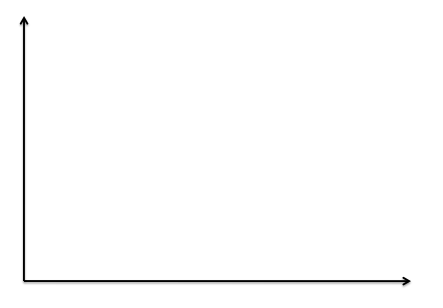
\includegraphics{axes.png}
	\end{adjustbox}
\end{center}

Alternatively, what if we could decrease $c$ for some workers? In this case, we would observe some of those workers switch to attending school. Let's define two groups - a treatment group $T$ which receives a decrease in the cost of schooling, and a control group $C$ which doesn't. Consider estimating
$$ \frac{\overline{w(S(T))} - \overline{w(S(C))}}{\overline{S(T)} - \overline{S(C)}} $$
We can estimate the average difference in wages between the two groups, and divide that by the average difference in schooling between the two groups. If $c$ is the only thing that changed, then the only reason wages are different between the two groups is the increased educational attainment of the treatment group. Therefore, this ratio will recover the effect of an increase in schooling on wages.

\begin{center}
	\begin{adjustbox}{
			max width=0.65\textwidth,
		}
		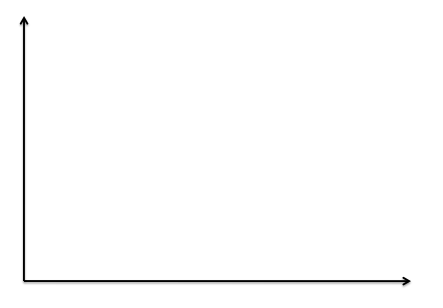
\includegraphics{axes.png}
	\end{adjustbox}
\end{center}

What if we don't have random assignment to treatment, as is the case with school construction in Indonesia? In that case, we can think about implementing a DID design - instead of using wages and schooling in the control group as the counterfactual for wages and schooling in the treatment group, we can use changes in wages and schooling in the control group as the counterfactual for changes in wages and schooling in the treatment group.
$$ \frac{\left(\overline{w(S(T,1))} - \overline{w(S(T,0))}\right) - \left(\overline{w(S(C,1))} - \overline{w(S(C,0))}\right)}{\left(\overline{S(T,1)} - \overline{S(T,0)}\right) - \left(\overline{S(C,1)} - \overline{S(C,0)}\right)} $$

Again, if the only reason wages in the treatment group broke from the trend of wages in the control group was the increase in schooling driven by the policy, then this will allow us to estimate the returns to schooling.

When using this to estimate the returns to schooling, we now need to ask two questions of the research design. First, is our parallel trends assumption valid? In other words, is it reasonable to assume that the treatment and control groups would have had the same trends in wages and schooling if the policy didn't happen? Second, did the policy only affect wages through changes in educational attainment?

To briefly recall, Duflo (2001) implements this methodology by comparing young relative to old cohorts in Indonesian districts that did and did not receive school construction in the late 1970's and early 1980's. Using this methodology, she finds that the construction caused a 0.12 increase in years of schooling, and about a 0.010-0.015 increase in log wages. Dividing the second by the first, this implies a returns to schooling of about 0.1 -- increasing average years of schooling by one year would cause a 10\% increase in wages. This surprisingly is similar to the .08 we estimated using the cross-country data.

To construct this estimate of 10\%, there are two fundamental assumptions. First, we need the estimates of the change in school attendance and the change in wages to be valid. In other words, we need to assume that, absent the school construction policy, the differences in wages across cohorts and in years of schoolings across cohorts would have been the same in treatment and control districts. As we mentioned, the selection of which districts received schools could confound this, especially if younger cohorts were adapting more rapidly to the rapid changes occurring in Indonesia at the same time as the school construction.

Second, we need to assume that the policy only affected wages through years of schooling. In other words, we need to assume that if the policy did not affect years of schooling, it would not have affected wages. For example, we need to assume that there was no direct effects of the infrastructure on wages, or effects on wages through improved educational quality.

\section{General equilibrium (Duflo (2004), Khanna (2016))}

Ideally, the question we would like to ask is ``should we build more schools'', or more generally ``how important is reducing the cost of attending school''. Can we just use our estimate of 10\% to answer these questions?

Maybe not. First, the private benefits and the societal benefits to attending school may be very different. School may not actually increase productivity of workers directly -- instead, it may be used as a signal of ability that employers use to more efficiently screen workers. Second, if labor demand of unskilled workers and skilled workers is downward sloping, then schooling, by converting unskilled workers into skilled workers, will increase the wage of unskilled workers and decrease the wage of skilled workers. Third, changes in the composition of workers may affect flows of capital between districts. For example, an increase in the number of skilled workers in one district might cause an increase in the construction of call centers. Fourth, the individuals that responded to the policy might have unusually high returns to schooling. If we expanded a similar policy, we might be worried that other individuals have much lower returns to schooling. Fifth, the districts targeted by this program might have unusually high returns to schooling -- in that case, although we'll estimate the returns to schooling in those districts, expanding the program to other districts may yield smaller results.

How can one address these critiques? (4) and (5) are both in general difficult. We can see if some districts appear to have much larger responses than others. Alternatively, we can look for estimates from different contexts and approaches to see the extent to which different estimates are consistent. (3) is also difficult -- it argues that positive effects in one districts may result in negative effects in other districts if those districts compete for investment. Hopefully, by focusing on medium run effects (5-10 years after the first beneficiaries of the program complete primary school), these changes in investment will not have taken place yet. However, (1) and (2) both suggest that old workers may not be a good control group for young workers. In particular, old workers may also see their wages change, as would other young workers. These multiple simultaneous changes may make the estimated effect hard to interpret. Ideally, if we had random assignment of districts to the program, we would be able to estimate these effects separately.

Khanna (2016) attempts to do that by studying a primary school construction program in India. Rather than using a DID, he instead uses the fact that eligibility for the program was determined by a hard cutoff for women's literacy in 1991. By comparing districts just above the cutoff to districts just below the cutoff, he claims that it's effectively random whether you end up just above or just below. This allows us to estimate the effects on not only educational attainment of the younger cohort, but also the wages of skilled and unskilled young and old workers separately.

He finds that these outcomes are affected in the expected ways -- an increase in the number of young workers attending school increases the wages of unskilled workers and decreases the wages of skilled workers, and these effects are magnified for young workers relative to old workers. However, accounting for all this, he estimates a social return to additional years of education that is very similar to the estimate from Duflo (2001), and his own estimate using the same DID estimation strategy as Duflo (2001) -- roughly 10\%.

Finally, should we care about the results of these studies at all? Both are effectively estimating the returns to primary school, since both focus on primary school construction. In most poor countries, primary school completion rates are approaching 100\%. In that sense, whether or not countries should have universal primary school completion is no longer considered an open policy question. However, the general question of the returns to schooling is still policy relevant -- lower and upper secondary and tertiary school completion rates are still low throughout the world. What will be the effect of increasing them? Additionally, as we'll ask going forward, what determines the returns to schooling? If quality of education is very low, then the returns to schooling may be very low as well. Documenting this, and understanding variation in the returns to schooling, remains important.

\end{document}